\section{使用集成工具获取鼠标光标的位置}

控制器运行后,按下 \lstinline{Ctrl} \lstinline{Alt} \lstinline{Shift} \lstinline{5},将集成工具切换到模式 5。

将鼠标光标移动到欲确定坐标的位置后,按下 \lstinline{Ctrl} \lstinline{Alt},罗技控制台中将输出鼠标光标的坐标位置。
为防止坐标输出过于频繁,因此每次输出鼠标光标位置后间隔 0.5 秒才会允许下一次输出鼠标光标位置。另外,若执行器当前处于暂停状态,则此功能也会被停用。

\begin{figure}[H]
    \Centering
    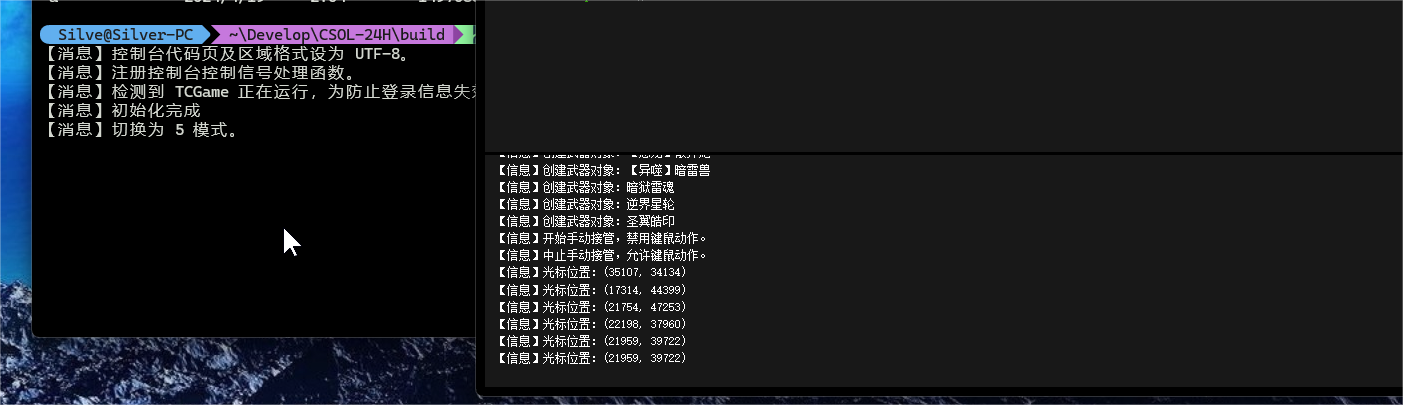
\includegraphics[width=\textwidth]{documents/assets/position.png}
    \caption{获取鼠标光标位置}
\end{figure}